\section{Verteilte Dateisysteme}

\subsection{Was ist ein verteiltes Dateisystem?}

Ein verteiltes Dateisystem ist ein Dateisystem, das die Speicherung von Daten auf mehrere Rechner verteilt. Dabei kann sowohl die Segmentierung von Daten, d.h. die Daten werden in verschiedene Bereiche unterteilt, wobei jeder Rechner einem anderen Bereich zugeordnet ist, als auch Replikation, d.h. mehrere Rechner speichern die selben Daten, um Ausfallsicherheit und andere Ziele von VS zu erreichen, vorliegen.

\subsubsection{Zugriffsmodelle}
\label{sec:zugriffsmodelle}
Wir unterscheiden zwischen den folgenden beiden Zugriffsmodellen verteilter Dateisysteme:
\begin{itemize}
    \item \textbf{Remote Access:}\\
          Hierbei finden alle schreibenden Zugriffe auf dem Server statt. Dazu ist eine komplexe Schnittstelle zwischen Client und Server nötig. Es entsteht eine dauerhafte Nutzung des Netzwerks mit kleinen Datenmengen
    \item \textbf{Upload/Download:}\\.
          Der Client kopiert zu Beginn eine Datei vom Server in seinen lokalen Speicher. Dann nimmt er dort Schreiboperationen vor und kopiert die Datei zurück auf den Server, wo sie dann gemerged wird. Die Schnittstelle, die benötigt wird ist also simpler. Das Netzwerk wird nur beim Öffnen und Schließen (impliziert download und upload) benötigt, dabei werden aber möglicherweise große Datenmengen übertragen.
\end{itemize}

\subsubsection{Schnittstellen-Design}
Eine wesentliche Eigenschaft der Schnittstelle eines verteilten Dateisystems ist, ob es zustandslos oder zustandsbehaftet ist.
\begin{itemize}
    \item \textbf{Zustandslos:}\\
          \begin{itemize}
              \item Im Server wird kein Speicher für den Status der Client-Verbindungen benötigt. Alle Informationen werden stattdessen in jedem Aufruf (jeder Nachricht) übertragen.
              \item Es gibt keine Operationen zum Öffnen oder Schließen von Dateien.
              \item Fehlertoleranter und einfacher zu implementieren, da nicht mit Verbindungsabbrüchen umgegangen werden muss.
          \end{itemize}
    \item \textbf{Zustandsbehaftet:}\\
          \begin{itemize}
              \item Nachrichten werden kürzer, da gewisse Informationen schon implizit im Verbindungsstatus vorliegen.
              \item Precaching möglich, da in Mitten einer Session schon bekannt ist, auf welche Datei ein Client zugreifen möchte.
              \item Locks (Sperren) sind einfach zu realisieren.
          \end{itemize}
\end{itemize}

\subsection{Network File System - NFS v4}

Das Network File System ist ein Netzwerkprotokoll, das implementiert werden kann, um ein verteiltes Dateisystem zu implementieren. Der Zugriff auf Dateien erfolgt für den Benutzer genau so, als ob die Dateien lokal gespeichert wären. NFS hat folgende Eigenschaften
\begin{itemize}
    \item NFS v4 ist \textbf{zustandsbehaftet}. Eine Datei wird mit verschiedenen Aufrufen geöffnet, gelesen geschrieben, geschlossen usw.. Die Vorgängerversion NFS v3 war allerdings zustandslos.
    \item Die \hyperref[sec:zugriffsmodelle]{Zugriffsart} ist \textbf{Remote-Access}.
    \item Die Änderungssemantik ist \textbf{Sitzungssemantik}. Das heißt, dass Änderungen an Dateien beim schließen der Datei sichtbar werden.
\end{itemize}

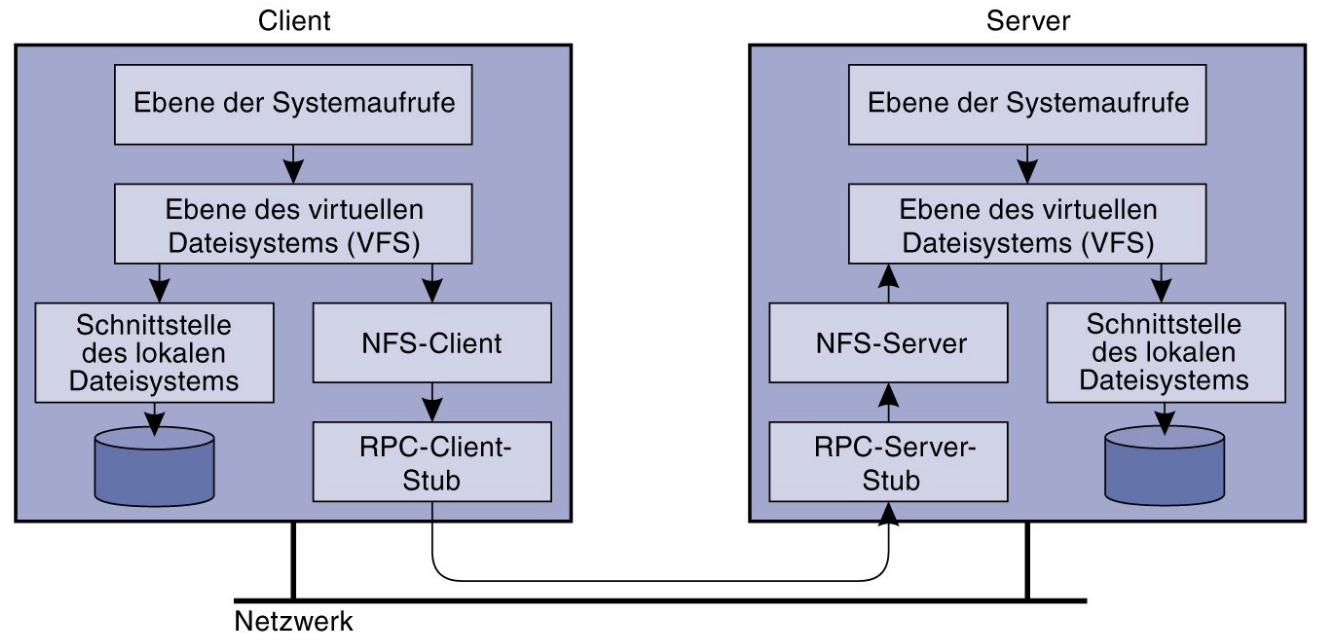
\includegraphics[height=150px]{nfs-architecture.png}


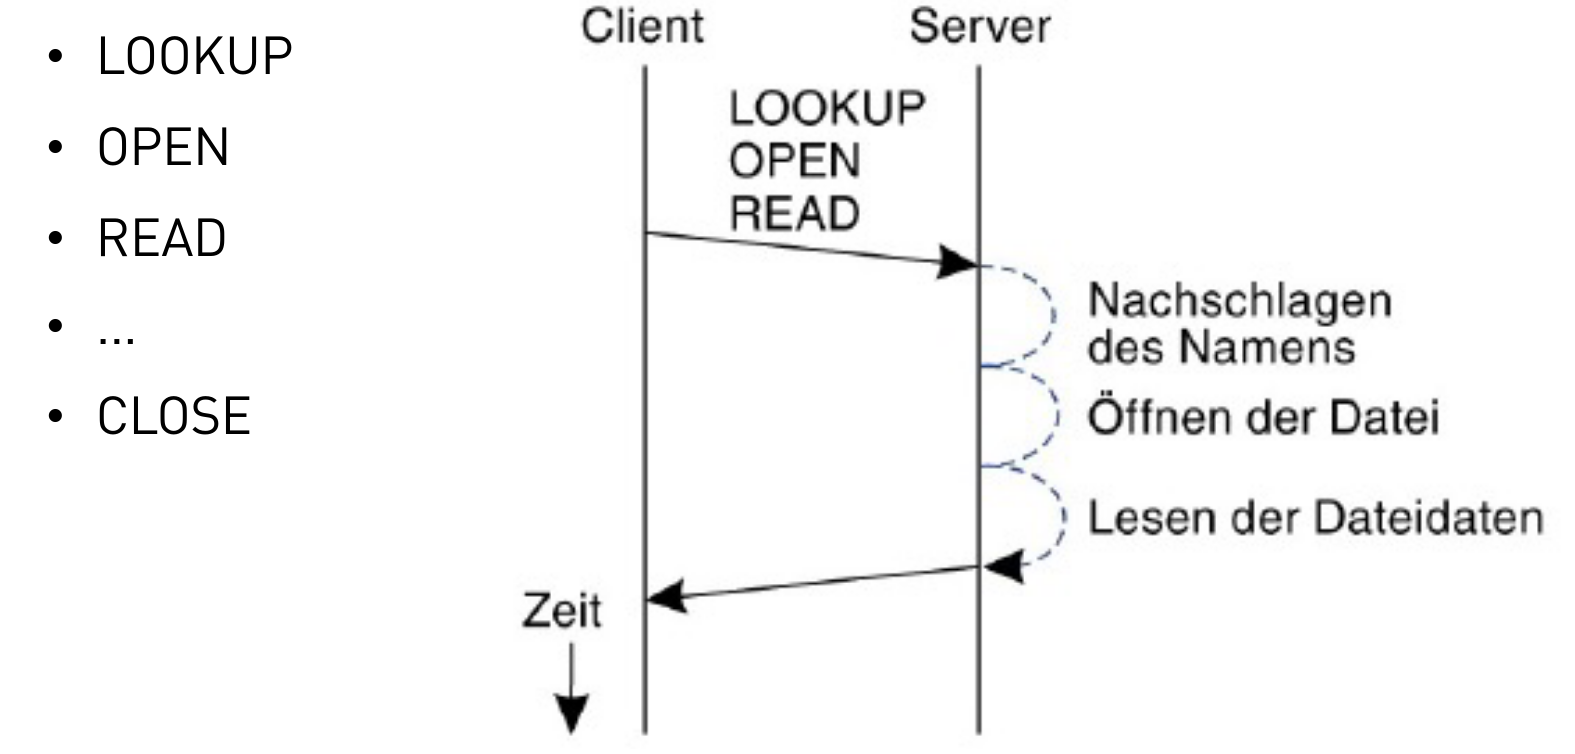
\includegraphics[height=150px]{nfs-sequence.png}

NFS basiert auf RPC. NFS v4 erlaubt es in einem RPC-Call mehrere Funktionsaufrufe zu übertragen. Im oberen Beispiel sehen wir z.B. wie ein LOOKUP, ein OPEN und ein READ zusammen übertragen werden, ausgeführt werden und dann nur das Gesamtergebnis zurückgeliefert wird.
\begin{itemize}
    \item \textbf{LOOKUP} liefert zunächst alle Server auf denen eine bestimmte Datei existiert.
    \item \textbf{READ} übernimmt eine Startposition und eine Anzahl an Bytes. Der Server wird dann diese Daten zurückliefern. Allerdings kann der Server auch weniger Daten zurückliefern, falls er der Meinung ist, dass die angefragte Datenmenge zu groß für einen einzigen RPC-Call ist.
\end{itemize}

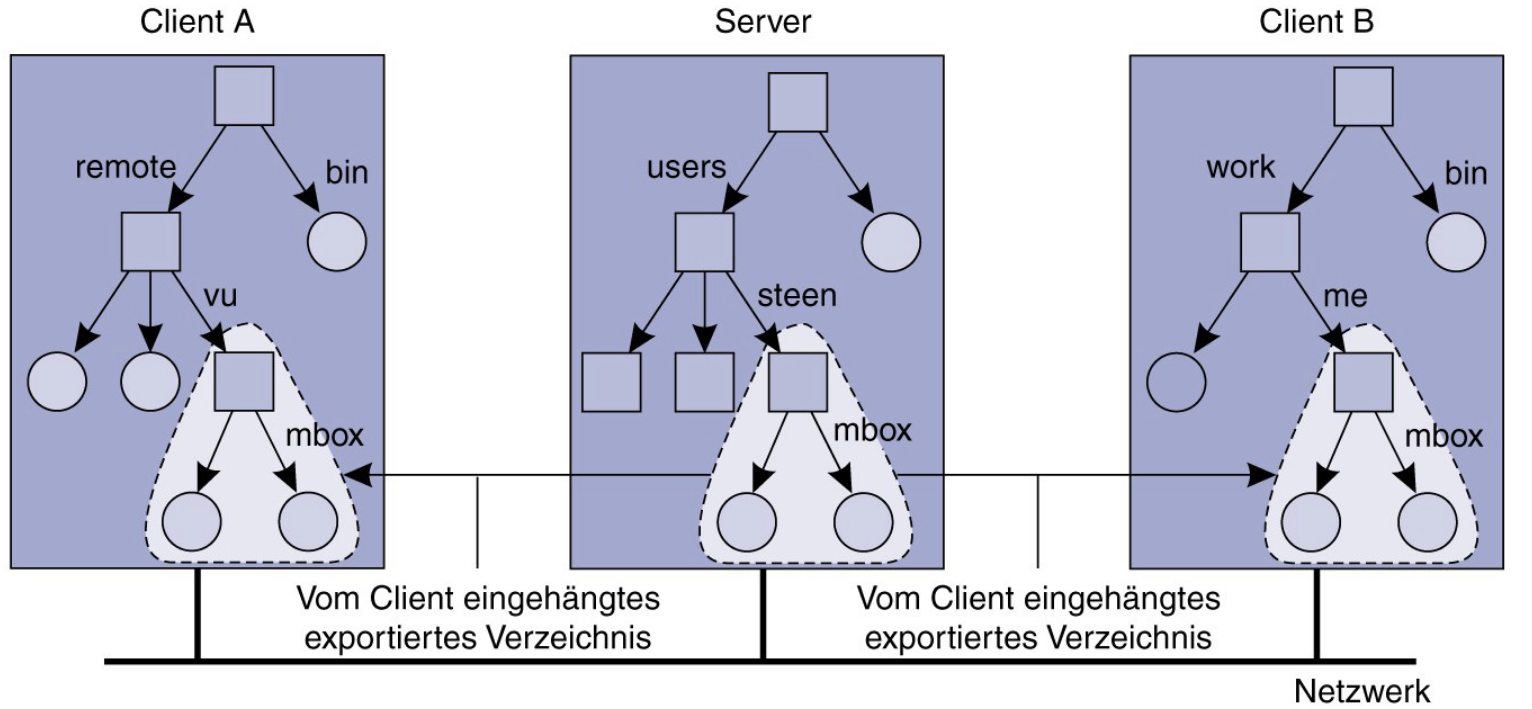
\includegraphics[height=150px]{nfs-mounting.png}

Um das verteilte Dateisystem in das eigene lokale Dateisystem einzubinden, kann es in den lokalen Verzeichnisbaum gemountet werden.

\subsubsection*{Locks}

NFS v4 ermöglicht es auch Sperren zu setzen. Man kann sowohl Schreib- als auch Lesesperren setzen. Durch diese Maßnahmen kann die Konsistenz des Systems durch den Benutzer bei kritischen Operationen sichergestellt werden.

\subsection{Google File System - GFS}
\label{sec:gfs}

Das Google File System ist ein von Google entwickeltes verteiltes Dateisystem, das auf Linux-Rechnern einsetzbar ist. Es ist auf große Datenmengen mit großen Dateien (über 100GB) optimiert. Der Haupteinsatzzweck ist die Verwendung im Zusammenhang mit Map-Reduce Operationen auf Basis von Suchanfragen. Bei der Entwicklung des Systems wurden folgende Annahmen gemacht:
\begin{itemize}
    \item Die Dateien sind enorm groß.
    \item Es gibt enorm viele Dateien.
    \item Das System wird von handelsüblichen Rechnern gehosted, die häufig ausfallen können.
    \item Dateien werden entweder gelesen oder es werden Daten angehängt. Das Ändern oder Löschen von bestehenden Daten kommt äußerst selten vor.
    \item Bandbreite ist wichtiger als Latenz, da große Datenmengen übertragen werden.
\end{itemize}

\subsubsection*{Systemdesign}

Dateien werden in mehrere 64MB große Chunks unterteilt. Jeder Chunk kann durch eine eindeutige ID, das chunk handle, identifiziert werden. Diese Chunks können dann auf mehrere Rechner aufgeteilt werden, sodass eine Datei nicht komplett auf einem einzigen Server liegen muss. Im GFS gibt es 2 Komponenten:
\begin{itemize}
    \item Einen \textbf{Master-Server:}\\
          Der Master Server speichert Metainformationen über den Zustand des Systems. Er weiß, welche Dateien es gibt, welche Chunks auf welchen Servern liegen und wie groß die Dateien sind. Diese Information bekommt er über zyklisches Abfragen aller Chunk-Server, die sogenannten Heart-Beat-Messages. Alle Anfragen von Clients, sowohl lesende als auch schreibende, laufen über diesen Master. Er liefert dem Client dann das chunk handle und die Adresse des zuständigen Chunk-Servers. Dann kann der Client seine Anfrage direkt an den Chunk-Server stellen. Damit der Master-Server nicht zum Bottleneck oder zur Schwachstelle werden kann, gibt es sogenannte Shadow-Master. Die Shadow-Master übernehmen zusätzlich die Koordination von Leseanfragen und springen für den richtigen Master-Server ein (siehe \hyperref[sec:fail-over-cluster]{Fail-Over-Cluster}).
    \item Sehr viele \textbf{Chunk-Server:}\\
          Die Chunk Server speichern einen ihnen zugewiesenen Teil der Chunks lokal in einem Linux-Dateisystem. Um Ausfallsicherheit zu gewährleisten, werden die Daten repliziert, sodass jeder Chunk auf mindestens 3 Chunk-Servern gespeichert ist. Jedem Chunk wird vom Master-Server ein bestimmter Chunk-Server als primary replica zugeordnet. Schreiboperationen werden dann zuerst auf dem primary replica ausgeführt und von dort aus mit einem \hyperref[sec:2pc]{2-Phasen-Commit} mit den anderen Chunk-Servern synchronisiert. Leseoperationen können auf jedem beliebigen Chunk durchgeführt werden, da diese Chunks durch die Synchronisierung mittels 2PC alle konsistent sein sollten. Das verfahren ist also ein \hyperref[sec:quorums]{Quorum} mit QW=n und QR=1. Hierbei entspricht n aber der Anzahl der Server auf denen das Chunk repliziert ist, also mindestens 3, und nicht der Anzahl der Gesamtrechner.
\end{itemize}

GFS verfolgt also eine \hyperref[sec:master-slave]{Master-Slave-Architektur}

\subsection{Andrew File System - AFS}

Das AFS ist ein verteiltes Dateisystem, das für die Carnegie Mellon University mit dem Fokus auf Skalierbarkeit entwickelt wurde. Es basiert auf RPC und wird auch im WAN genutzt.

\subsection{Hadoop Distributed File System - HDFS}

Das Hadoop Distributed File System ist ein verteiltes Dateisystem, das Teil von Apache Hadoop ist und daher speziell für \hyperref[sec:map-reduce]{Map-Reduce} optimiert ist. Es ist ähnlich aufgebaut wie das \hyperref[sec:gfs]{GFS}.